\documentclass[a4paper]{scrartcl}
\usepackage{mathtools}
\usepackage{titlesec}
\usepackage[utf8]{inputenc}
\usepackage[polish]{babel}
\usepackage{textcomp}
\usepackage[T1]{fontenc}
\usepackage{amsthm}
\usepackage{amsfonts}
\usepackage{graphicx}

\title{Warsztaty 2}
\author{Dawid Żywczak}
\date{31 marca 2020}

\begin{document}
\maketitle

\begin{figure}
  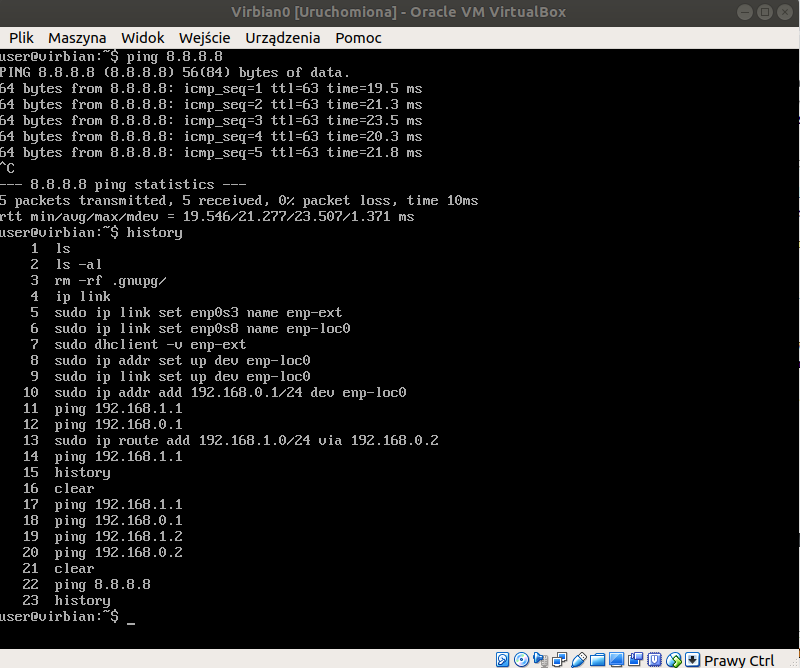
\includegraphics[width=\linewidth]{hv1.png}
  \caption{Historia terminala z maszyny Virbian0}
  \label{fig:hv1}
\end{figure}

\begin{figure}
  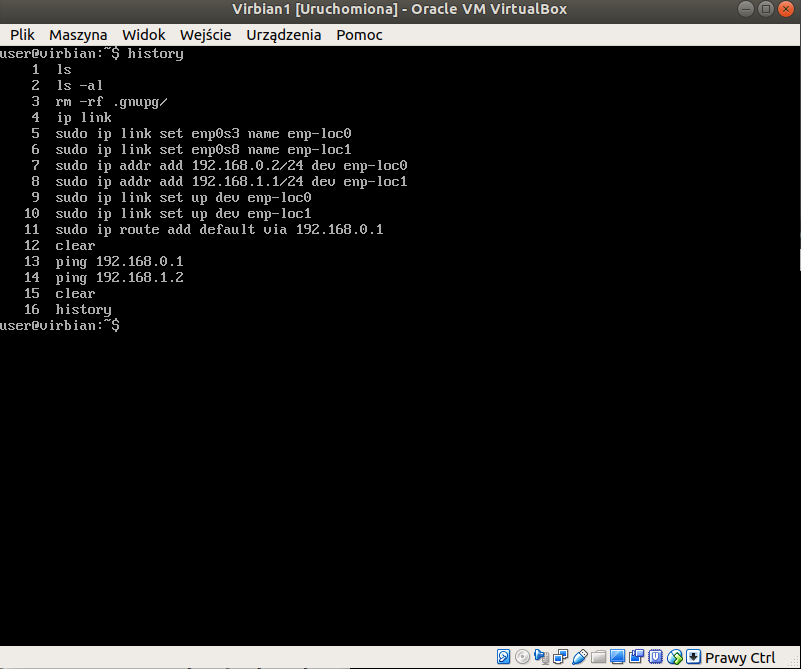
\includegraphics[width=\linewidth]{hw2.png}
  \caption{Historia terminala z maszyny Virbian1}
  \label{fig:hv2}
\end{figure}

\begin{figure}
  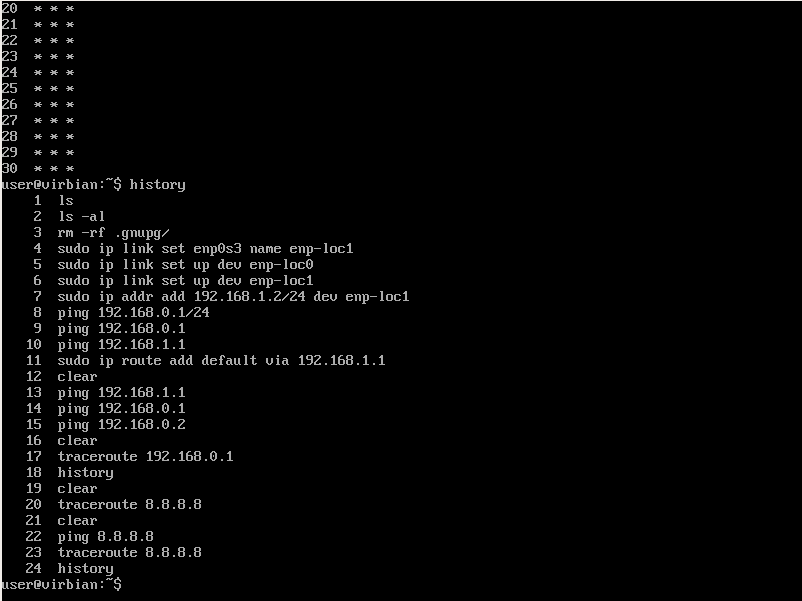
\includegraphics[width=\linewidth]{hw33.png}
  \caption{Historia terminala z maszyny Virbian2}
  \label{fig:hv3}
\end{figure}

\begin{figure}
  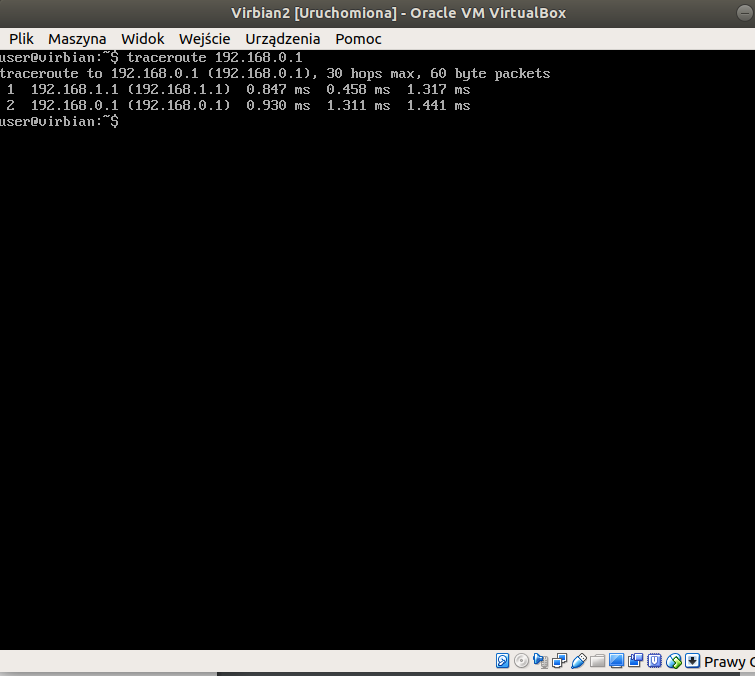
\includegraphics[width=\linewidth]{traceroute.png}
  \caption{Program traceroute uruchomiony z Virbiana2 do Virbiana0}
  \label{fig:tr}
\end{figure}

\begin{figure}
  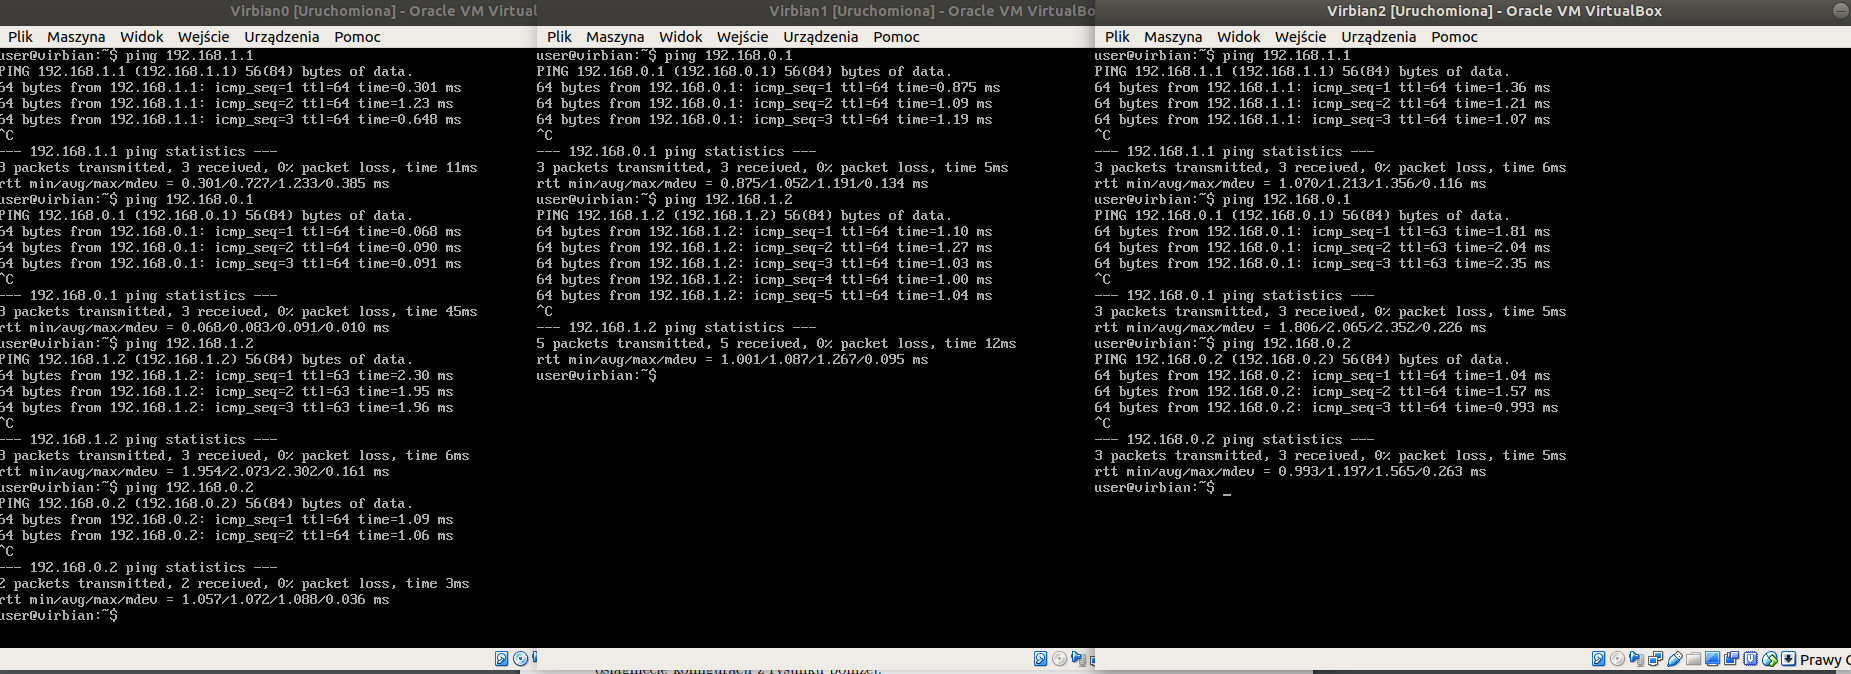
\includegraphics[width=\linewidth]{pings.png}
  \caption{Sprawdzenie osiągalności wszystkich interfejsów}
  \label{fig:tr}
\end{figure}

\begin{figure}
  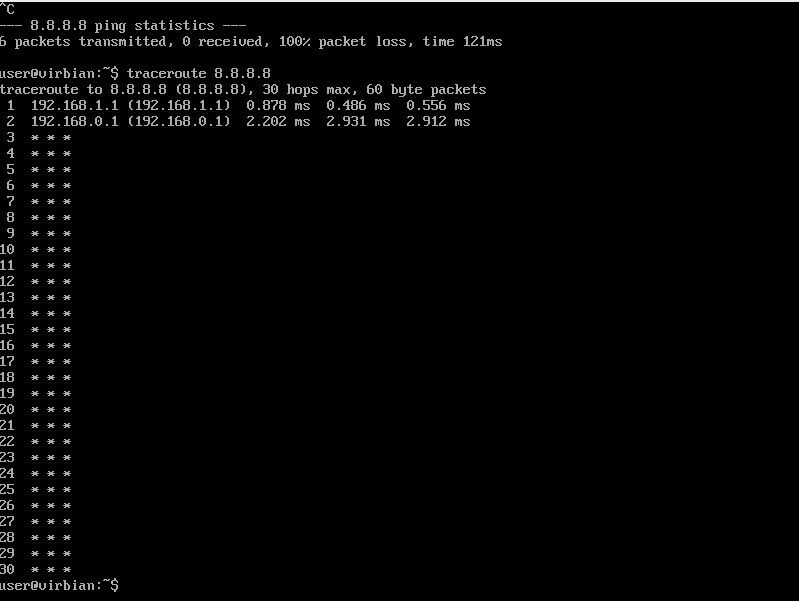
\includegraphics[width=\linewidth]{hw3.png}
  \caption{Zjawisko braku odpowiedzi na pinga 8.8.8.8 z Virbiana2}
  \label{fig:error}
\end{figure}
Nie wiedziałem do końca w jaki sposób przekazać Panu odpowiedzi oraz dowody na wykonanie zadania, więc umieściłem zrzuty ekranu historii poszczególnych maszyn wirtualnych. Co do ostatniego punktu zadania: Wydaje mi się, że jest to spowodowane faktem, że interfejs NAT wykonuje translację adresów sieciowych, przez co zatracana jest informacja, gdzie należy odesłać odebrany pakiet. Wydaje mi się, że żeby to naprawić, musielibyśmy powiadomić zewnętrzne sieci, do których coś wysyłamy, o swojej wewnętrznej konfiguracji sieciowej. Zewnętrzne sieci nie mają pojęcia o istnieniu maszyny Virbian2, więc nawet, gdybyśmy w Virbian0 ustawili w jaki sposób traktować pakiety do Virbiana2, to niewiele by dało.

\end{document}
